\documentclass[UTF8,a4paper,11pt]{ctexart}

\usepackage[margin=2.2cm]{geometry}
\usepackage{amsmath}
\usepackage{amssymb}
\usepackage{array}
\usepackage{booktabs}
\usepackage{longtable}
\usepackage{xcolor}
\usepackage{listings}
\usepackage[most]{tcolorbox}
\usepackage{hyperref}
\usepackage{tikz}
\usetikzlibrary{arrows.meta,positioning,calc,shapes.geometric,decorations.markings}

\hypersetup{colorlinks=true, linkcolor=blue!60!black, urlcolor=blue!60!black,
            pdfborder=0 0 0}

\lstset{
  basicstyle=\ttfamily\small,
  breaklines=true,
  frame=single,
  rulecolor=\color{black!30},
  numberstyle=\tiny\color{black!60},
  keywordstyle=\color{blue!60!black}\bfseries,
  commentstyle=\color{black!50}\itshape,
  language=C
}

\newcommand{\reg}[1]{\texttt{#1}}
\newcommand{\code}[1]{\texttt{#1}}

\newtcolorbox{intuition}[1][直觉]{
  enhanced, breakable, colback=blue!4, colframe=blue!50!black,
  fonttitle=\bfseries, title=#1, sharp corners=south,
  boxrule=0.5pt, left=4pt, right=4pt, top=2pt, bottom=2pt
}
\newtcolorbox{trap}[1][踩坑提醒]{
  enhanced, breakable, colback=red!4, colframe=red!60!black,
  fonttitle=\bfseries, title=#1, sharp corners=south,
  boxrule=0.5pt, left=4pt, right=4pt, top=2pt, bottom=2pt
}
\newtcolorbox{example}[1][数值示范]{
  enhanced, breakable, colback=green!4, colframe=green!50!black,
  fonttitle=\bfseries, title=#1, sharp corners=south,
  boxrule=0.5pt, left=4pt, right=4pt, top=2pt, bottom=2pt
}

\title{在 TX32F01 上手搓一颗 FOC \\ \large 架构、原理与全过程数值走查}
\author{基于 \texttt{APP\_FOC/} 工程整理}
\date{\today}

\begin{document}
\maketitle

\begin{abstract}
本文目标只有一个：让一个 \emph{从来没做过 FOC} 的嵌入式工程师，读完后能讲清楚
\texttt{APP\_FOC} 工程里每一段代码 \emph{为什么这样写}。所以前半部分几乎不写公式，
全部用图和类比；公式推导集中放在后半，并附一个 \textbf{把真实数字一路喂下去走完
整条流水线} 的例子，便于自己单步对照。
\end{abstract}

\tableofcontents
\bigskip

%======================================================================
\section{5 分钟看懂 FOC}
%======================================================================

\subsection{我们到底要把电机当什么用？}

\textbf{直流有刷电机} 的好处是：你给它通多少电流，它就出多少力矩，几乎线性。坏处是
有碳刷会磨损。\textbf{无刷电机（BLDC / PMSM）} 把碳刷换成电子换向，可靠了，但代价是
三相电流之间是 \emph{耦合} 的，给定输入电流跟力矩之间不再是简单的比例关系。

\textbf{FOC 的全部目的}：用数学把无刷电机重新"伪装"成直流有刷电机。在 FOC 控制器
内部存在一个虚拟的旋转坐标系，电机在这个坐标系里看起来就是一个普通直流电机，
有"励磁电流 $i_d$"和"力矩电流 $i_q$"两根独立的旋钮。控制器只管转这两个旋钮，外面再
反变换回三相电压扔给逆变器。

\begin{intuition}
"FOC = 用软件给无刷电机戴一副旋转眼镜，让它在眼镜里看起来像直流电机，然后用 PI
控直流电机就完事了。"
\end{intuition}

\subsection{整条信号链一图流}

\begin{center}
\begin{tikzpicture}[node distance=6mm and 8mm,
                    every node/.style={font=\small},
                    blk/.style={draw, rounded corners=2pt, minimum width=18mm,
                                minimum height=8mm, fill=blue!8, align=center},
                    sblk/.style={blk, fill=green!10},
                    out/.style={blk, fill=orange!15},
                    arr/.style={-{Stealth[length=2mm]}, thick}]
  \node[sblk]                       (adc)    {ADC\\$i_a, i_b$};
  \node[sblk, right=of adc]         (clarke) {Clarke\\$i_\alpha,i_\beta$};
  \node[sblk, right=of clarke]      (park)   {Park\\$i_d, i_q$};
  \node[sblk, right=of park]        (pi)     {PI\\$v_d, v_q$};
  \node[out,  below=of pi]          (ipark)  {Inv Park\\$v_\alpha,v_\beta$};
  \node[out,  left=of ipark]        (svpwm)  {SVPWM\\$t_a,t_b,t_c$};
  \node[out,  left=of svpwm]        (pwm)    {3$\times$ PWM\\TIM0/1/2};
  \node[blk, left=of pwm, fill=yellow!20] (motor) {Motor\\+ 桥};
  \node[blk, below=10mm of motor, fill=yellow!20] (hall) {Hall};
  \draw[arr] (adc)    -- (clarke);
  \draw[arr] (clarke) -- (park);
  \draw[arr] (park)   -- (pi);
  \draw[arr] (pi)     -- (ipark);
  \draw[arr] (ipark)  -- (svpwm);
  \draw[arr] (svpwm)  -- (pwm);
  \draw[arr] (pwm)    -- (motor);
  \draw[arr] (motor)  -- (hall);
  \draw[arr] (hall.east) -| node[pos=0.7,right,font=\scriptsize]{$\theta$}
             ($(park.south)+(0,-1mm)$) -- (park.south);
  \draw[arr, dashed] (motor.south) |- node[pos=0.7,below,font=\scriptsize]{shunt}
             ($(adc.south)+(0,-3mm)$) -- (adc.south);
\end{tikzpicture}
\end{center}

绿色块是 \textbf{前向（测量 $\to$ 状态）}，橙色块是 \textbf{后向（指令 $\to$ 输出）}，
中间夹一个 PI。这一整圈 10\,kHz 跑一次，全部在 ADC EOC 中断里完成。

\subsection{每一块到底在干什么}

\begin{itemize}
  \item \textbf{ADC}：电流采样。两路下桥串联的 shunt 把电流转成电压，运放放大后送进
        ADC。\emph{为什么只测两相？}—— 三相之和为零，第三相可推。
  \item \textbf{Clarke}：把三个 120$^\circ$ 互错的相电流，等价地"投影"到一个 XY 平面
        $(\alpha,\beta)$。本质上只是从冗余的 3D 表达换到自由度真正只有 2 的 2D 表达。
  \item \textbf{Park}：让 $(\alpha,\beta)$ 这副坐标系跟着转子一起转。\emph{在跟转子
        同步的坐标系里，原本以电频率振荡的正弦电流变成了恒定的直流值。}
  \item \textbf{PI}：在直流量上做 PI 控制，零稳态误差，调参也简单。
  \item \textbf{Inv Park}：PI 输出的 $(v_d, v_q)$ 是在"旋转眼镜里"看到的指令电压，要变
        回静止坐标系才能驱动真正的硬件。
  \item \textbf{SVPWM}：把 $(v_\alpha, v_\beta)$ 翻译成三路 PWM 占空比，并通过共模注入把
        母线利用率从 50\% 提到 86.6\%。
  \item \textbf{Hall}：告诉我们转子现在的角度 $\theta$，让 Park 的"旋转眼镜"知道该转
        到哪一格。
\end{itemize}

\subsection{为什么不直接控三相电流？}

可以，叫"滞环控制"或者"三相 PI"。问题：

\begin{itemize}
  \item 电机在转，三相电流是 50/100/500\,Hz 的交流。PI 在交流量上有稳态相位差和幅值差，
        响应越快越糟。
  \item 三相之间互相耦合，一相变化会影响另一相，PI 参数互相打架。
\end{itemize}

FOC 跳到 dq 旋转坐标系之后，PI 看到的全是直流，没耦合，没稳态误差，整定一次终身用。
这是 FOC 比"六步换向"贵 100 倍代码却被广泛采用的原因。

%======================================================================
\section{硬件资源分配}
%======================================================================

\subsection{时钟与定时器算账}

系统时钟 $f_\text{SYS} = 24\,\text{MHz}$，定时器通过 \reg{DIV} 寄存器分频：

\[
  f_\text{TIM} = \frac{f_\text{SYS}}{\text{DIV}+1} = \frac{24}{3} = 8\,\text{MHz}
\]

PWM 频率取 $f_\text{PWM} = 10\,\text{kHz}$，所以 \reg{ARR}（自动重装载）

\[
  \text{ARR} = \frac{f_\text{TIM}}{f_\text{PWM}} - 1 = 799
\]

每个 PWM 周期 $T_\text{PWM} = 100\,\mu\text{s}$，即 \textbf{每秒 1 万次完整 FOC 回路}。
死区时间 $T_d$ 直接以 tick 数写入 \reg{DTG}：默认 20 tick $= 2.5\,\mu\text{s}$。

\begin{intuition}
PWM 频率怎么选？太低（< 8\,kHz）会让人耳听见啸叫；太高（> 30\,kHz）开关损耗大、
DT 占比高。8 -- 20\,kHz 是工业 BLDC 的甜区，TX32F01 在 10\,kHz 跑得很轻松。
\end{intuition}

\subsection{为什么用三个定时器？}

TX32F01 的库每个 TIM 只暴露 \emph{一对} OCx/OCxN 互补输出。三相全桥要三对，所以
TIM0、TIM1、TIM2 各扛一相。三个定时器 ARR 设成相同值，启动时把 CR.CEN 在几条指令内
连续置位，三个载波之间的相位差只有几个时钟，FOC 完全感知不到。

\begin{table}[h]
\centering
\caption{三相 PWM 引脚映射（见 \texttt{foc\_config.h}）}
\begin{tabular}{lccccc}
\toprule
相 & 定时器 & 上桥 (OCx) & 下桥 (OCxN) & 上桥 AF & 下桥 AF \\
\midrule
U & TIM0 & GPIO2.PIN02 & GPIO0.PIN03 & T0CH & T0CHN \\
V & TIM1 & GPIO0.PIN00 & GPIO0.PIN01 & T1CH & T1CHN \\
W & TIM2 & GPIO1.PIN05 & GPIO1.PIN04 & T2CH & T2CHN \\
\bottomrule
\end{tabular}
\end{table}

\subsection{ADC 怎么接到 PWM 上}

\reg{ADC.CFGR.TRGSEL} 设为 Timer0，TIM0 的 update 事件自动启动 ADC 序列。序列长度 3，
依次采 $i_a, i_b, V_\text{bus}$。整条序列完成 EOC 触发中断，FOC 主回路就在这个 ISR 里
跑——\textbf{不需要主循环参与节拍管理}。

\begin{center}
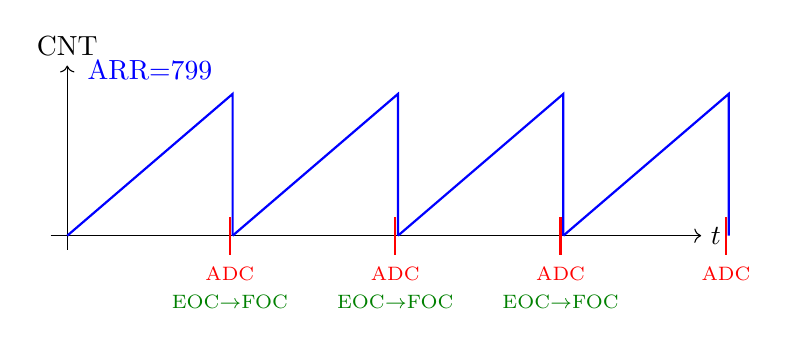
\begin{tikzpicture}[xscale=0.7, yscale=0.6]
  % PWM carrier (sawtooth)
  \draw[->] (-0.3,0)--(11.5,0) node[right]{$t$};
  \draw[->] (0,-0.3)--(0,3.6) node[above]{CNT};
  \foreach \i in {0,...,3} {
    \draw[blue, thick] (\i*3,0) -- ({\i*3+3},3) -- ({\i*3+3},0);
  }
  \node[blue] at (1.5,3.5) {ARR=799};
  % ADC sample marks
  \foreach \i in {0,1,2,3} {
    \draw[red, thick] ({\i*3+3-0.05},-0.4)--({\i*3+3-0.05},0.4);
    \node[red, font=\scriptsize] at ({\i*3+3-0.05},-0.8) {ADC};
  }
  % FOC label
  \foreach \i in {1,2,3} {
    \node[green!50!black, font=\scriptsize] at ({\i*3-0.05},-1.4) {EOC$\to$FOC};
  }
\end{tikzpicture}
\end{center}

每 100\,$\mu$s：TIM0 计到顶 $\to$ update 事件 $\to$ 启动 ADC $\to$ 8\,$\mu$s 后 EOC
中断 $\to$ 跑 FOC（约 25\,$\mu$s） $\to$ 写新 CCR $\to$ 下一周期立即生效。

\subsection{Hall 怎么接}

三路 Hall 信号分别挂三个 EXTI 线，双边沿触发，三个 IRQ 入口都指向同一个
\code{hall\_isr()}。中断里只做两件事：

\begin{enumerate}
  \item 读三个 GPIO 拼出 3-bit Hall 码；
  \item 查表把 Hall 码翻译成扇区中心角，更新 \code{s\_angle}。
\end{enumerate}

整个 ISR 不到 50 cycle。

%======================================================================
\section{Clarke 变换：从三个变量到两个变量}
%======================================================================

\subsection{为什么三相只用两个变量就够}

电机是三相无中线接法，物理约束：

\[
  i_a + i_b + i_c = 0
\]

三个量有一个等式约束，自由度其实只有 2。所以信息完整地放在一个 2D 平面里完全够，
没必要拖着三个量做后续运算。

\subsection{两种"投影"方式：等幅 vs 等功率}

把 a、b、c 三根坐标轴想象成在平面内相隔 120$^\circ$ 的三个方向，三相电流就是沿
这三个方向的"位移"。它们的合成就是一个 2D 平面上的矢量 $\vec{i}$。Clarke 变换就是把
这个矢量用直角坐标系 $(\alpha, \beta)$ 表达。

\begin{center}
\begin{tikzpicture}[scale=1.1]
  \draw[->] (-2,0)--(2.4,0) node[right]{$\alpha$};
  \draw[->] (0,-1.6)--(0,1.8) node[above]{$\beta$};
  % 三相轴
  \draw[->, blue!70!black, thick] (0,0)--(2,0) node[right]{$a$ 轴};
  \draw[->, blue!70!black, thick] (0,0)--(-1, 1.732) node[above left]{$b$ 轴};
  \draw[->, blue!70!black, thick] (0,0)--(-1,-1.732) node[below left]{$c$ 轴};
  % 例子矢量
  \draw[->, red, very thick] (0,0)--(1.2, 0.8) node[right]{$\vec i$};
  \draw[dashed, red!60] (1.2,0)--(1.2,0.8);
  \draw[dashed, red!60] (0,0.8)--(1.2,0.8);
  \node[red, font=\scriptsize] at (1.3,-0.18) {$i_\alpha$};
  \node[red, font=\scriptsize] at (-0.18,0.85) {$i_\beta$};
\end{tikzpicture}
\end{center}

\textbf{等幅形式}（amplitude-invariant，我们用的版本）：

\[
  \begin{bmatrix} i_\alpha \\ i_\beta \end{bmatrix}
  = \frac{2}{3}
  \begin{bmatrix} 1 & -\tfrac12 & -\tfrac12 \\ 0 & \tfrac{\sqrt3}{2} & -\tfrac{\sqrt3}{2} \end{bmatrix}
  \begin{bmatrix} i_a \\ i_b \\ i_c \end{bmatrix}
\]

\textbf{等功率形式}（power-invariant）只是把上面的 $\tfrac{2}{3}$ 换成 $\sqrt{\tfrac{2}{3}}$，
让 $|\vec{i_{\alpha\beta}}|^2 = |\vec{i_{abc}}|^2$。控制工程一般用等幅形式（更直观），
信号处理课本经常用等功率形式（数学更对称）。

\subsection{利用 $i_a+i_b+i_c=0$ 简化成只需两路 ADC}

把 $i_c = -i_a - i_b$ 代入，化简：

\[
\boxed{
  \;i_\alpha = i_a,\qquad
  i_\beta  = \frac{1}{\sqrt 3}(i_a + 2 i_b)\;
}
\]

这就是 \code{foc\_math.c::foc\_clarke()} 里两行的内容。常数 $1/\sqrt{3}$ 在 Q15 下写作
\code{Q15\_INV\_SQRT3 = 18919}。

\begin{example}
设 $i_a = +1.0$\,A, $i_b = -0.5$\,A：
\begin{align*}
i_\alpha &= 1.0\,\text{A} \\
i_\beta  &= (1.0 + 2 \cdot (-0.5))/\sqrt 3 = 0/\sqrt 3 = 0
\end{align*}
矢量 $\vec i$ 完全在 $\alpha$ 轴上——符合直觉：当 $i_b$ 是 $i_a$ 的 $-1/2$，
说明 $i_c = -0.5$ 也是 $-1/2$，三相处在 $i_a$ 为正、$i_b/i_c$ 各分担一半负电流的对称
状态，矢量自然指向 $a$ 轴方向。
\end{example}

%======================================================================
\section{Park 变换：戴上旋转眼镜}
%======================================================================

\subsection{为什么要再换一次坐标系}

经过 Clarke 之后，$i_\alpha, i_\beta$ 仍然是 \emph{交流量}——电机在转，相量也在
$\alpha\beta$ 平面里画圈圈。PI 控制器在交流量上有稳态误差。怎么办？

\textbf{把坐标系也转起来，跟着相量一起转。} 这就是 Park 变换。

\begin{center}
\begin{tikzpicture}[scale=1.2]
  \draw[->] (-2,0)--(2.5,0) node[right]{$\alpha$};
  \draw[->] (0,-1.6)--(0,1.8) node[above]{$\beta$};
  % 旋转中的 dq 坐标系
  \pgfmathsetmacro{\T}{32}
  \draw[->, orange!80!black, very thick]
       (0,0) -- ({1.8*cos(\T)},{1.8*sin(\T)}) node[right]{$d$ 轴};
  \draw[->, orange!80!black, very thick]
       (0,0) -- ({-1.8*sin(\T)},{1.8*cos(\T)}) node[above]{$q$ 轴};
  \draw[orange!80!black] (0.6,0) arc (0:\T:0.6) node[midway, right, font=\scriptsize]{$\theta$};
  % 同一个电流矢量
  \draw[->, red, very thick] (0,0)--({1.5*cos(\T)+0.2*cos(\T+90)},{1.5*sin(\T)+0.2*sin(\T+90)})
                              node[above right]{$\vec i$};
\end{tikzpicture}
\end{center}

\begin{intuition}
$d$（direct，直轴）指向转子 N 极方向；$q$（quadrature，交轴）和 $d$ 垂直，超前 90$^\circ$。
"沿着 $d$ 轴的电流不出力（只产生磁场），沿着 $q$ 轴的电流才出力矩"。所以 FOC 的标准
玩法是让 $i_d^* = 0$，全部电流都用来出力，效率最高。
\end{intuition}

\subsection{Park 公式}

数学上就是一个 2D 旋转矩阵，把 $(\alpha,\beta)$ 转 $-\theta$ 度变成 $(d,q)$：

\[
  \begin{bmatrix} i_d \\ i_q \end{bmatrix}
  =
  \begin{bmatrix} \cos\theta & \sin\theta \\ -\sin\theta & \cos\theta \end{bmatrix}
  \begin{bmatrix} i_\alpha \\ i_\beta \end{bmatrix}
\]

代码两行：

\begin{lstlisting}
*d = q15_mul(a, c) + q15_mul(b, s);   // i_d
*q = q15_mul(b, c) - q15_mul(a, s);   // i_q
\end{lstlisting}

\textbf{反 Park}（PI 输出反变换回静止坐标系）就是上式取转置：

\[
  \begin{bmatrix} v_\alpha \\ v_\beta \end{bmatrix}
  =
  \begin{bmatrix} \cos\theta & -\sin\theta \\ \sin\theta & \cos\theta \end{bmatrix}
  \begin{bmatrix} v_d \\ v_q \end{bmatrix}
\]

\subsection{$\theta$ 哪来？}

这是 FOC 工程化里最关键的一个问题。来源有三种：

\begin{itemize}
  \item \textbf{Hall}：6 个扇区 $\times$ 60$^\circ$，分辨率粗但便宜可靠。\emph{本工程用这个。}
  \item \textbf{编码器}：分辨率高、调试简单，但贵且占引脚。
  \item \textbf{无感}：从反电势 / 电流变化率反推，没传感器但低速下不准。
\end{itemize}

\begin{trap}
$\theta$ 一旦不准，PI 算出来的 $(v_d, v_q)$ 就被反 Park 错位地塞给电机，结果可能是
电机抽搐、嗡嗡叫、空转烫手。任何 FOC 故障的 95\% 都是 \textbf{角度对位错了}。
所以上电第一件事永远是：手动慢转转子，确认 Hall 扇区顺序符合预期。
\end{trap}

%======================================================================
\section{SVPWM：把电压指令塞进 PWM}
%======================================================================

\subsection{为什么不能直接做正弦 PWM}

最朴素的做法：把三相电压指令各自做 PWM 调制，每个相对应一个占空比 $d_x = (v_x + V_\text{bus}/2)/V_\text{bus}$。
\textbf{问题}：当 $|v_x| > V_\text{bus}/2$ 时，占空比超出 [0,1]，会被钳到 0 或 1，
电压幅值就到顶了。母线利用率上限：50\%。

SVPWM（Space Vector PWM）能让母线利用率提到 $\sqrt{3}/2 \approx 86.6\%$，比正弦 PWM 多
出 15\%。多出来的电压可以让电机在相同直流母线下转得更快、出力更大。

\subsection{标准 SVPWM 太复杂，min-mid-max 注入完全等价}

经典 SVPWM 要做 6 个扇区判断 + 矢量分解 + 零矢量分配，公式一堆。但下面这个等价做法
\textbf{只要 6 个比较、3 个加法}：

\begin{enumerate}
  \item 先用反 Clarke 算三相电压指令 $v_a, v_b, v_c$；
  \item 找出三者的 min 和 max，记 $v_n = (v_\text{min} + v_\text{max})/2$；
  \item 每相减去 $v_n$ 得到 $v_a', v_b', v_c'$；
  \item 把 $v_x'$ 从 $[-1, +1]$ 映射到 $[0, \text{ARR}+1]$ 就是占空比。
\end{enumerate}

\subsection{为什么"中点平移"等价于 SVPWM}

电机是三相无中线，所以给三相同时加一个 \emph{共模电压} 不会改变线电压，
也就不会改变电机看到的电流。这给了我们一个自由度：可以把三相电压同时"平移"。

把中位平移到母线中点，相当于把"最大相"和"最小相"对称分布在母线两端，浪费的余量
最少。可以证明这等价于标准 SVPWM 的零矢量分配。

\begin{center}
\begin{tikzpicture}[xscale=1.6, yscale=0.7]
  % 母线范围
  \draw[gray, dashed] (-0.3,1) -- (4.3,1) node[right, font=\scriptsize]{$+V_\text{bus}/2$};
  \draw[gray, dashed] (-0.3,-1) -- (4.3,-1) node[right, font=\scriptsize]{$-V_\text{bus}/2$};
  \draw[gray] (-0.3,0) -- (4.3,0);
  % 注入前
  \node at (0.5,-1.7) {\small 注入前（正弦 PWM）};
  \fill[red!60] (0.3,0.8) rectangle (0.7,0.85);
  \fill[red!60] (0.8,0.3) rectangle (1.2,0.35);
  \fill[red!60] (1.3,-0.4) rectangle (1.7,-0.35);
  \node[font=\tiny] at (0.5,0.95){$v_a$};
  \node[font=\tiny] at (1.0,0.45){$v_b$};
  \node[font=\tiny] at (1.5,-0.5){$v_c$};
  % 注入后
  \node at (3.3,-1.7) {\small 注入后（SVPWM 等价）};
  \fill[green!60!black] (2.9,0.6) rectangle (3.3,0.65);
  \fill[green!60!black] (3.4,0.1) rectangle (3.8,0.15);
  \fill[green!60!black] (3.9,-0.6) rectangle (4.3,-0.55);
  \node[font=\tiny] at (3.1,0.75){$v_a'$};
  \node[font=\tiny] at (3.6,0.25){$v_b'$};
  \node[font=\tiny] at (4.1,-0.7){$v_c'$};
  % 箭头
  \draw[->, thick] (2.0,0) -- (2.6,0) node[midway, above, font=\scriptsize]{$-v_n$};
\end{tikzpicture}
\end{center}

% 注入前最大幅 0.5；注入后最大幅 sqrt(3)/2 ≈ 0.866

\subsection{Cortex-M0 无除法怎么映射到占空比}

公式 \eqref{eq:duty}：

\[
  d_x = \frac{v_x' + 1}{2} \cdot N,\qquad N = \text{ARR}+1
  \label{eq:duty}
\]

要用除法，但 M0 没有硬件除。技巧：把 Q15 值（$-32768 \dots +32767$）加上 $32768$ 变成
uint16，再乘以 $N$，结果是 32-bit；然后右移 16 位代替除以 $65536$：

\begin{lstlisting}
uint32_t da = ((uint32_t)((int32_t)va + 32768) * period) >> 16;
\end{lstlisting}

\subsection{占空比 → CCR}

库里 OCx 的极性约定是：CNT=0 时初始为高（高桥导通），计到 CCR 时翻低。
所以高电平持续时间 $t_\text{on} = N - \text{CCR}$，反过来：

\[
\boxed{\;\text{CCR} = N - d_x\;}
\]

这就是 \code{foc\_pwm\_commit()} 那一行：\code{ccr\_a = period\_p1 - t\_a;}

%======================================================================
\section{PI 控制器：FOC 唯一可以"调参"的部分}
%======================================================================

\subsection{为什么 dq 坐标系下 PI 这么好用}

经过 Clarke + Park 之后，$i_d, i_q$ 在稳态下是 \emph{直流}。直流上 PI 没有稳态误差，
带宽好定，没有相位差。这就是为什么 FOC 的电流环只需 PI 而不需要 PID 或更复杂的控制律。

\subsection{离散形式（Backward Euler）}

\begin{align*}
u_p(k) &= K_p \cdot e(k) \\
u_i(k) &= u_i(k-1) + K_i \cdot e(k) \\
u(k)   &= u_p(k) + u_i(k)
\end{align*}

注意 $K_i$ 已经吸收了采样周期 $T_s$，所以代码里没有单独乘 $T_s$。

\subsection{抗饱和：条件积分法}

如果电压输出已经顶到了 $V_\text{bus}/2$，再让积分继续累积就是"积分饱和"，事后退饱和
会有明显超调。处理方法：

\begin{lstlisting}
int32_t i_step = q15_mul(err, p->ki);
int32_t inew   = p->integ + i_step;
int32_t out    = q15_mul(err, p->kp) + inew;
if (out > p->out_max) { out = p->out_max; if (i_step > 0) inew = p->integ; }
else if (out < p->out_min) { out = p->out_min; if (i_step < 0) inew = p->integ; }
p->integ = inew;
\end{lstlisting}

\textbf{条件积分}：只在输出还没饱和、或饱和方向相反时，才更新积分项。代价几乎为零，
效果接近完整的 anti-windup。

\subsection{调参顺序}

\begin{enumerate}
  \item \textbf{$K_p$}：先把 $K_i = 0$，逐渐加大 $K_p$ 直到 $i_q$ 阶跃响应出现轻微振荡，
        然后降回 70\%。
  \item \textbf{$K_i$}：从一个小值开始（$K_p / 100$ 量级），增大到稳态误差在 1$\sim$2 步内
        消除即可。再大就会让响应变得"软"。
  \item \textbf{$d$ 轴和 $q$ 轴} 用同一组增益，电机的 $L_d$ 和 $L_q$ 差异不大的情况下
        够用了。表贴 PMSM、BLDC 全部如此。
\end{enumerate}

%======================================================================
\section{Hall 角度估计}
%======================================================================

\subsection{6 个有效状态对应 6 个扇区}

120$^\circ$ 间隔的三个 Hall 传感器在电机转一圈电气角中输出 6 个不同的 3-bit 码。
0b000 和 0b111 是无效状态（传感器开路或短路）。剩下 6 个对应 6 个 60$^\circ$ 扇区：

\begin{center}
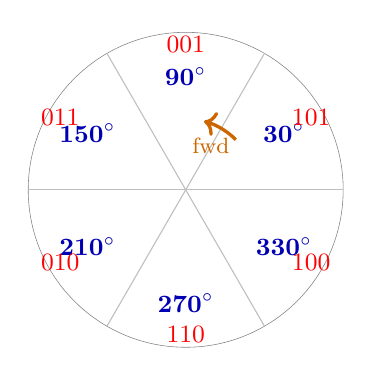
\begin{tikzpicture}[scale=2]
  \draw[gray, very thin] (0,0) circle (1);
  \foreach \i in {0,60,120,180,240,300} {
    \draw[gray!50] (0,0) -- ({\i}:1);
  }
  % 扇区中心 + Hall 码
  \node[blue!70!black, font=\small\bfseries] at ( 30:0.72) {30$^\circ$};
  \node[red,           font=\small]           at ( 30:0.92) {101};
  \node[blue!70!black, font=\small\bfseries] at ( 90:0.72) {90$^\circ$};
  \node[red,           font=\small]           at ( 90:0.92) {001};
  \node[blue!70!black, font=\small\bfseries] at (150:0.72) {150$^\circ$};
  \node[red,           font=\small]           at (150:0.92) {011};
  \node[blue!70!black, font=\small\bfseries] at (210:0.72) {210$^\circ$};
  \node[red,           font=\small]           at (210:0.92) {010};
  \node[blue!70!black, font=\small\bfseries] at (270:0.72) {270$^\circ$};
  \node[red,           font=\small]           at (270:0.92) {110};
  \node[blue!70!black, font=\small\bfseries] at (330:0.72) {330$^\circ$};
  \node[red,           font=\small]           at (330:0.92) {100};
  % 旋转方向箭头
  \draw[->, very thick, orange!80!black] (45:0.45) arc (45:75:0.45);
  \node[orange!80!black, font=\footnotesize] at (60:0.32) {fwd};
\end{tikzpicture}
\end{center}

\subsection{角度怎么用整数表示}

代码里电角度用 \code{uint16\_t}：$0 \to 0^\circ$，$65535 \to \approx 360^\circ$。
30$^\circ$ 在这种表示下就是 $\lfloor 65536 \cdot 30/360 \rfloor = 5461$，其他类推。
查表常数见 \code{foc\_hall.c::s\_sector\_center[]}。

\subsection{速度估计：边沿间隔法}

相邻两次 Hall 边沿之间正好走过一个扇区（60$^\circ = \pi/3$）。如果中间经过了 $n$ 个
PWM 周期（每个 $T_\text{PWM} = 100\,\mu\text{s}$），则电角速度：

\[
  \omega_e = \frac{\pi/3}{n \cdot T_\text{PWM}} = \frac{\pi f_\text{PWM}}{3 n}
\]

换算到机械转速（极对数 $P$）：

\[
  \text{RPM} = \frac{60 \omega_e}{2\pi P} = \frac{10 f_\text{PWM}}{n P}
\]

\begin{example}
极对数 $P=4$，相邻 Hall 边沿间隔 $n=50$ 个 PWM 周期：
$\text{RPM} = (10 \times 10000) / (50 \times 4) = 500$ RPM。
\end{example}

%======================================================================
\section{走一遍完整周期 —— 用真实数字}
%======================================================================

假设此刻：转子电角度 $\theta = 60^\circ$（uint16 = 10923），目标 $i_d^* = 0$，
$i_q^* = +5000$ (Q15，对应额定力矩的约 15\%)。ADC 测到 $i_a = +0.3$\,A，$i_b = -0.1$\,A
（标定后转 Q15 后约 \code{ia\_q15 = 4915}, \code{ib\_q15 = -1638}）。

\subsection*{Step 1 — Clarke}
\begin{align*}
i_\alpha &= 4915 \\
i_\beta  &= (4915 + 2 \cdot (-1638))/\sqrt 3 = 1639/\sqrt 3 \approx 946
\end{align*}

\subsection*{Step 2 — sin/cos 查表}
$\theta = 10923 \Rightarrow$ 索引 $\lfloor 10923 / 256 \rfloor = 42$，
查表得 $\sin \approx 28377$ ($\sqrt 3/2$), $\cos \approx 16384$ ($1/2$)。

\subsection*{Step 3 — Park}
\begin{align*}
i_d &= 4915 \cdot \tfrac{16384}{32768} + 946 \cdot \tfrac{28377}{32768}
     \approx 2458 + 819 = 3277 \\
i_q &= 946 \cdot \tfrac{16384}{32768} - 4915 \cdot \tfrac{28377}{32768}
     \approx 473 - 4258 = -3785
\end{align*}

\subsection*{Step 4 — PI}

误差 $e_d = 0 - 3277 = -3277$，$e_q = 5000 - (-3785) = 8785$。\\
比例项 $u_{p,d} = 0.1 \times -3277 = -328$；$u_{p,q} = 0.1 \times 8785 = 878$。\\
积分项（假设 $K_i = 0.005$，初始 $u_i = 0$）：$u_{i,d} = -16$，$u_{i,q} = +44$。\\
输出：$v_d = -344$, $v_q = 922$。

\subsection*{Step 5 — 反 Park}
\begin{align*}
v_\alpha &= -344 \cdot \tfrac{16384}{32768} - 922 \cdot \tfrac{28377}{32768}
          \approx -172 - 799 = -971 \\
v_\beta  &= -344 \cdot \tfrac{28377}{32768} + 922 \cdot \tfrac{16384}{32768}
          \approx -298 + 461 = 163
\end{align*}

\subsection*{Step 6 — 反 Clarke}
\begin{align*}
v_a &= v_\alpha = -971 \\
v_b &= -971/2 + (\sqrt 3/2) \cdot 163 \approx -486 + 141 = -345 \\
v_c &= -971/2 - (\sqrt 3/2) \cdot 163 \approx -486 - 141 = -627
\end{align*}

\subsection*{Step 7 — min-mid-max 注入}

$v_\text{min} = -971$（$v_a$），$v_\text{max} = -345$（$v_b$）。\\
$v_n = (-971 + -345)/2 = -658$。\\
注入后：$v_a' = -313$, $v_b' = 313$, $v_c' = 31$。

\subsection*{Step 8 — 占空比}

$N = 800$, $d_x = (v_x' + 32768) \cdot 800 / 65536$：

\begin{align*}
d_a &= (-313 + 32768) \cdot 800 / 65536 \approx 396 \\
d_b &= ( 313 + 32768) \cdot 800 / 65536 \approx 404 \\
d_c &= (  31 + 32768) \cdot 800 / 65536 \approx 400
\end{align*}

\subsection*{Step 9 — CCR}

\begin{align*}
\text{CCR}_0 &= 800 - 396 = 404 \\
\text{CCR}_1 &= 800 - 404 = 396 \\
\text{CCR}_2 &= 800 - 400 = 400
\end{align*}

下一个 PWM 周期：U 相高电平 396 tick，V 相高电平 404 tick，W 相高电平 400 tick。
线电压 $v_{ab} = (404-396) \cdot V_\text{bus}/800 \approx +1\% V_\text{bus}$。

\begin{intuition}
注意结果：三相 duty 都在 50\% 附近，差异只有 1\%——是因为我们这一拍的指令很小
（5000/32768 $\approx$ 15\%）。如果指令变大，三个 duty 会拉开到 [2.5\%, 97.5\%] 之间。
\end{intuition}

%======================================================================
\section{时序与中断预算}
%======================================================================

一个 PWM 周期 100\,$\mu$s = 2400 cycle @ 24\,MHz。一次完整 FOC 主回路开销：

\begin{table}[h]
\centering
\begin{tabular}{lr}
\toprule
模块 & cycles \\
\midrule
ADC 读 3 个 DR + 偏置减法     & $\sim$30 \\
sin/cos 查表（两次）          & $\sim$30 \\
Clarke 变换                   & $\sim$30 \\
Park（4 次乘加）              & $\sim$40 \\
PI $\times$ 2（含抗饱和）     & $\sim$80 \\
反 Park（4 次乘加）           & $\sim$40 \\
SVPWM (min-mid-max + 缩放)    & $\sim$120 \\
3 次 CCR 写入                 & $\sim$15 \\
中断进出 + 软向量转发         & $\sim$200 \\
\midrule
\textbf{合计}                 & $\sim$600 \\
\bottomrule
\end{tabular}
\end{table}

剩余 1800 cycle 给：Hall ISR（约 50 cycle）、SysTick（约 100 cycle）、主循环 shell。
\code{foc\_loop.c} 用 \reg{SysTick.VAL} 在每次 ISR 入口/出口测量真实开销，存到
\code{g\_foc.max\_loop\_cyc}，shell 的 \code{tel} 命令打印。

%======================================================================
\section{安全设计}
%======================================================================

\subsection{死区时间}

互补输出之间必须留死区，否则上下桥同时导通会瞬间烧 MOSFET。\code{TIM\_SetDeadTime()}
写入 \reg{DTG} 寄存器，单位是定时器 tick。默认 \code{FOC\_DEADTIME\_TCK = 20}
$\approx 2.5\,\mu\text{s}$，对普通栅极驱动器（如 IR2104）足够。

\begin{trap}
死区时间不能凭直觉设。\textbf{至少要等于 MOSFET 关断延迟 + 驱动器传播延迟}。
不确定就先 \textbf{在示波器上看互补波形}，确认上下桥之间确实有一段 dead-zone 才上电流。
\end{trap}

\subsection{硬件过流：Break Input}

把比较器输出接 TIMER\_BRK\_IN（GPIO1.PIN02），下降沿触发后 BDTR 硬件强制把所有
OCx/OCxN 拉到预设安全电平。这条路 \textbf{不经过 CPU}，延迟只有几个 tick，比软件
保护快得多。

\subsection{占空比上下钳位}

SVPWM 输出钳位到 $[\text{DT}, N - \text{DT}]$，避免极端占空比下死区把脉冲"吃光"产生
窄脉冲。在 10\,kHz / ARR=799 / DT=20 下，duty 限幅 $\approx [2.5\%, 97.5\%]$，对调速性
能没有可见影响。

\subsection{无 VTOR 软向量}

TX32F01（Cortex-M0）没有 VTOR，所有真实中断都由 Bootloader 在 0x01000000 接管。
\code{APP\_FOC} 通过 \code{app\_softvec\_register\_irq()} 把 FOC ISR 等注册到 SRAM
0x20000000 的软向量表，Bootloader trampoline 转发过来——每次中断多约 7 cycle，
对 600 cycle 的回路来说可忽略。

%======================================================================
\section{文件总览}
%======================================================================

\begin{table}[h]
\centering
\begin{tabular}{ll}
\toprule
文件 & 作用 \\
\midrule
\code{FOC/foc\_config.h}    & 引脚映射、PWM 频率、PI 增益、死区时间 \\
\code{FOC/foc\_math.h/.c}   & Q15 sin/cos 表、Clarke/Park/IPark、PI、SVPWM \\
\code{FOC/foc\_pwm.h/.c}    & 三定时器同步启动 + 互补输出 + 死区时间 \\
\code{FOC/foc\_adc.h/.c}    & 三通道序列采样 + EOC ISR 调度 FOC 回路 \\
\code{FOC/foc\_hall.h/.c}   & EXTI 双边沿、扇区中心锁定、速度估计 \\
\code{FOC/foc\_loop.h/.c}   & 模式机：idle / align / V/F / 闭环 FOC \\
\code{FOC/foc\_shell.h/.c}  & 非阻塞 UART REPL + 100 ms telemetry \\
\code{USER/main.c}          & 上电时序、ADC 零点校准、主循环节拍 \\
\bottomrule
\end{tabular}
\end{table}

%======================================================================
\section{常见错误与现象速查表}
%======================================================================

\begin{table}[h]
\centering
\small
\begin{tabular}{p{5cm}p{8cm}}
\toprule
现象 & 大概率原因 \\
\midrule
电机抽搐 / 嗡嗡叫，转不起来 & 角度对位错了。慢手转，确认 Hall 码顺序为 5-1-3-2-6-4。 \\
电机能转但有一边特别费力   & 一相接反了，或 Hall 通道顺序对调了。 \\
低速顺畅高速发抖           & 死区补偿没做，或 Hall 边沿间隔噪声大，加 EXTI 滤波。 \\
通电瞬间烧管               & 死区时间太短，或 Break 没接，或下桥默认电平不对。 \\
$i_q$ 上升后掉一半         & ADC 饱和。检查 shunt 阻值 + 运放增益 + ADC 量程匹配。 \\
PI 永远调不到零稳态        & 积分被钳了。检查 \code{out\_max/min} 设得是否够大。 \\
转速越高 $i_q$ 跟踪越差    & 没加反电势前馈 $\omega L_q i_q$，或电感模型不准。 \\
Hall 码偶发跳 0 或 7       & 滤波不够，加 EXTI 软件去抖动或硬件 RC。 \\
\bottomrule
\end{tabular}
\end{table}

%======================================================================
\section{下一步可以做什么}
%======================================================================

\begin{enumerate}
  \item \textbf{无感 FOC}：把 Hall 模块换成 SMO 或 SoGI-PLL，利用反电势估角度；
        M0 上要小心收敛速度与噪声放大。
  \item \textbf{外环转速 / 位置 PID}：当前只有电流环 + Hall 速度反馈骨架。
  \item \textbf{单电阻采样}：母线单电阻 + 时序重构相电流，省运放和 ADC 通道，
        但要重新规划 ADC 触发相位。
  \item \textbf{增益调度}：转速分段切换 PI 参数，或加前馈 $\omega L_d i_d / \omega L_q i_q$，
        高速下电流跟踪明显改善。
  \item \textbf{故障日志}：把过流、过压、Hall 异常事件写入 \code{APP\_LOG}，方便现场
        定位。
  \item \textbf{上位机调参}：参考 VOFA+ 的 JustFloat 协议，固件加 30 行就能实时画
        $i_d/i_q/i_a/i_b$ 波形。
\end{enumerate}

%======================================================================
\appendix
%======================================================================
\section{Q15 定点速查}

\begin{itemize}
  \item 数值范围：$[-1, +1) \leftrightarrow [-32768, 32767]$ (int16)
  \item 乘法：$a \cdot b \to ((a \cdot b) + 2^{14}) \gg 15$
  \item 加法：直接加，需要溢出 saturate
  \item 除以 2：算术右移 1（注意负数舍入）
  \item Sin/Cos：256 步全周期，1/4 周期 64 项表 + 三段对称展开
\end{itemize}

\section{常用 Q15 常数}

\begin{tabular}{ll}
\toprule
常数 & Q15 值 \\
\midrule
$1$           & 32767 \\
$1/2$         & 16384 \\
$\sqrt 3/2$   & 28377 \\
$1/\sqrt 3$   & 18919 \\
$2/\sqrt 3$   & 37837（超出 Q15，需用 32-bit 中间） \\
\bottomrule
\end{tabular}

\section{Hall 上电对位流程}

\begin{enumerate}
  \item shell 输入 \code{idle}，确认 PWM 50/50/50，无电流。
  \item 手缓慢顺时针转动转子一圈，观察 \code{tel} 的 \code{h=} 字段，
        应按 5 $\to$ 1 $\to$ 3 $\to$ 2 $\to$ 6 $\to$ 4 循环。
  \item 顺序不对：调换电机任意两根相线（或两根 Hall 线），
        \textbf{不要} 改源代码里的 \code{s\_sector\_center[]}——那是行业标准映射。
  \item 输入 \code{align}，200\,ms 后转子应自锁到电角度 0；
        放手再缓慢转，\code{th=} 字段应连续滑过 0 $\to$ 0x1556 $\to$ 0x4000 $\to$ ……
\end{enumerate}

\end{document}
